\chapter{PLANTEAMIENTO DEL PROBLEMA}
\section{Descripción de la Realidad Problemática}

En América Latina, la situación es igualmente preocupante. Un estudio realizado por la Comisión Económica para América Latina y el Caribe (CEPAL) reveló que el 60\% de los habitantes rurales no tienen acceso a servicios de salud adecuados \citep*{OECD_World_Bank_2020}. La falta de acceso a servicios de salud tiene consecuencias graves para la población pediátrica. La UNICEF informa que las tasas de mortalidad infantil en áreas rurales son significativamente más altas que en áreas urbanas. En países en desarrollo, los niños que viven en zonas rurales tienen el doble de probabilidades de morir antes de los cinco años en comparación con sus contrapartes urbanas \cite{UNICEF}.

La situación de atención médica en las áreas rurales de Perú es una realidad compleja y desafiante. Imagine comunidades enclavadas en paisajes montañosos y remotos, donde acceder a servicios médicos básicos es una odisea. La falta de infraestructura adecuada y la escasez de profesionales de la salud crean una brecha significativa en el acceso a la atención médica, dejando a muchas personas sin la ayuda que necesitan cuando más la necesitan. Según el Instituto Nacional de Estadística e Informática (INEI), en 2022, solo el 20\% pertenece a la población rural, en comparación con el 80\% de la población urbana. Esto significa que millones de peruanos en áreas rurales son más vulnerables a enfermedades y muertes evitables.

\begin{figure}[h]
	\begin{center}
		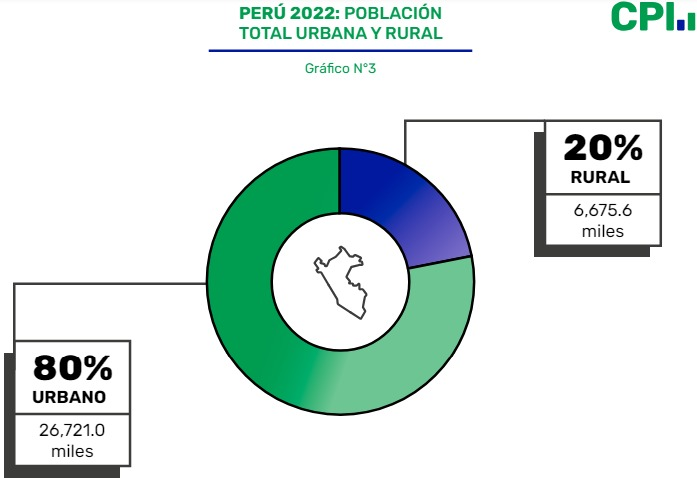
\includegraphics[width=0.6\textwidth]{1/figures/INEITOTAL.jpeg}
		\caption{Total de poblacion rural y urbana. Fuente: \cite{gl_inei}}
		\label{1:fig}
	\end{center}
\end{figure}

Ademas, los datos oficiales respaldan estas realidades duras. Según el Ministerio de Salud de Perú, en el 2021, más del 70\% de la población rural carecía de acceso regular a servicios médicos adecuados. Esto no es solo una estadística fría, sino una narrativa de vidas afectadas, enfermedades no tratadas y vidas que podrían haberse salvado con una atención médica oportuna.

\begin{figure}[h]
	\begin{center}
		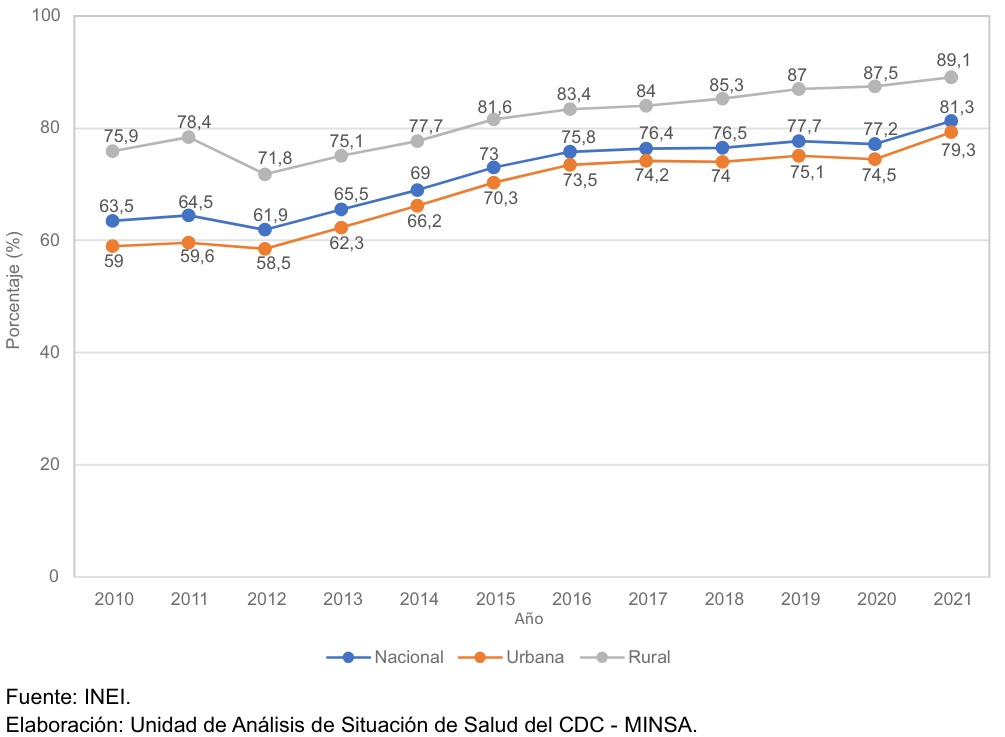
\includegraphics[width=0.6\textwidth]{1/figures/MINSA.jpeg}
		\caption{Porcentaje de acceso a atencion medica. Fuente: \cite{gl_inei}}
		\label{2:fig}
	\end{center}
\end{figure}
%\begin{figure}[h]
%	\begin{center}
	%		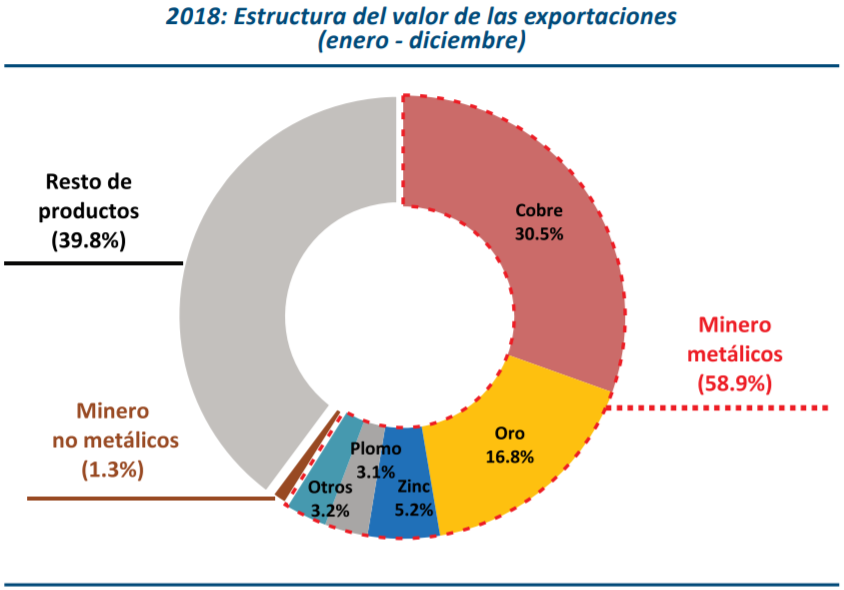
\includegraphics[width=0.8\textwidth]{1/figures/estructura_exportaciones_peru.png}
	%		\caption{Estructura del valor de las exportaciones peruanas en el año 2018. Fuente: \cite{cu_ministerioPeru_statsminas}}
	%		\label{1:fig2}
	%	\end{center}
%\end{figure}

Durante el período comprendido entre 2022 y 2024, la pandemia de COVID-19 solo ha intensificado estos desafíos. Los recursos y la atención se desplazaron hacia la respuesta a la pandemia, dejando otras necesidades de salud pública en segundo plano. Las comunidades rurales se encontraron aún más marginadas, enfrentando una atención médica aún más limitada y fragmentada.

Sin embargo, entre estas sombras de dificultades, hay un rayo de esperanza en la forma de la tecnología. El aumento del acceso a teléfonos móviles en áreas rurales ofrece una oportunidad única para brindar servicios médicos básicos a través de plataformas digitales, incluso en las zonas más remotas del país. Es aquí donde entra en juego la idea de un chatbot médico.

Imagínese un sistema donde las personas en las comunidades rurales pueden acceder a información médica básica, hacer consultas sobre síntomas y recibir orientación sobre cómo buscar atención médica, todo desde la comodidad de sus teléfonos móviles. Esto no solo podría salvar vidas, sino también aliviar la carga sobre los pocos centros de salud disponibles en estas áreas.

Pero, por supuesto, hay obstáculos por superar. La adaptación cultural, la capacitación de los usuarios y la garantía de la precisión de la información son solo algunos de los desafíos que enfrenta esta iniciativa. Además, la conectividad limitada en algunas áreas rurales plantea desafíos adicionales para garantizar un acceso efectivo a la aplicación.

La implementación de Chatbots Médicos en áreas rurales del Perú tiene el potencial de mejorar significativamente el acceso a la atención médica para millones de personas. Estos sistemas pueden proporcionar información y asesoramiento médico de manera remota, sin necesidad de que un médico esté presente físicamente. Además, los Chatbots Médicos pueden ayudar a los pacientes a programar citas, recordarles que tomen sus medicamentos y monitorear su progreso. 

%\begin{figure}[h]
%	\begin{center}
%		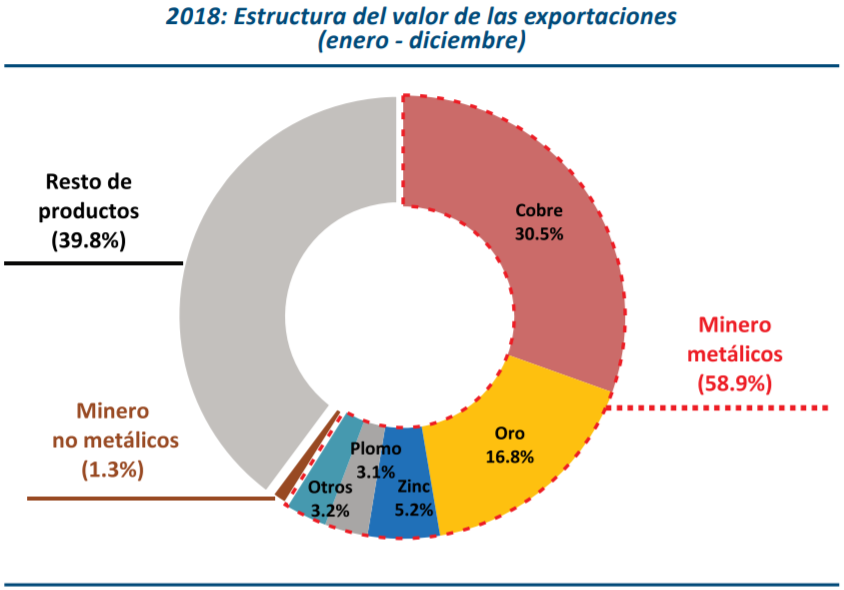
\includegraphics[width=0.8\textwidth]{1/figures/estructura_exportaciones_peru.png}
%		\caption{Estructura del valor de las exportaciones peruanas en el año 2018. Fuente: \cite{cu_ministerioPeru_statsminas}}
%		\label{1:fig2}
%	\end{center}
%\end{figure}

%\begin{figure}[h]
%	\begin{center}
%		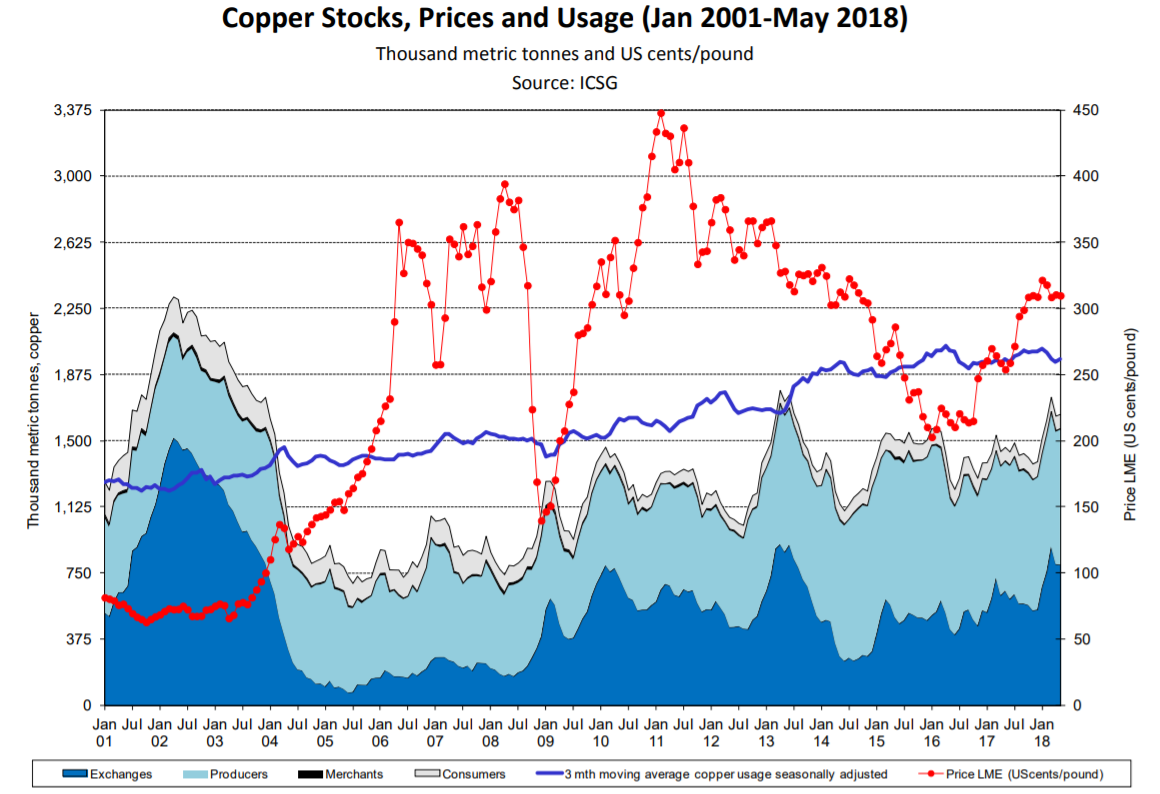
\includegraphics[width=0.8\textwidth]{1/figures/copper_stocks_prices_usage.png}
%		\caption{Precio, stocks y uso del cobre (cantidad en miles de toneladas y precio en centavos por libra). Fuente: \cite{cu_internationalcopper2018}}	
%		\label{1:fig3}
%	\end{center}
%\end{figure}

\section{Formulación del Problema}

%Para lefecto \parencite{ot_marti2018manual}. 


%Una vez elaborado el diagrama (véase Anexo 1), 

\subsection{Problema General}
\newcommand{\ProblemaGeneral}{
¿De qué manera la implementación de un chatbot médico puede mejorar el acceso a servicios de salud en las zonas rurales de Perú?
}
\ProblemaGeneral
\subsection{Problemas Espec\'{i}ficos}
\newcommand{\Pbone}{
¿Que datos disponibles se necesitaran para la implementacion de chatbot?
}
\newcommand{\Pbtwo}{
¿Que arquitectura podrían ser utilizadas para desarrollar un chatbot médico?
}
\newcommand{\Pbthree}{
¿Qué métodos de entrenamiento y validación se pueden utilizar para un chatbot?
}
\newcommand{\Pbfour}{
¿Qué métricas se pueden utilizar para evaluar la efectividad del chatbot médico?
}


\begin{itemize}
	\item \Pbone
	\item \Pbtwo
	\item \Pbthree
	\item \Pbfour

\end{itemize}

\section{Objetivos de la Investigación}

%Para la formulación de los objetivos de la presente investigación se elaboró un «árbol de objetivos» (véase Anexo 2) 
\subsection{Objetivo General}
\newcommand{\ObjetivoGeneral}{
Implementar un chatbot médico efectivo y sostenible para brindar servicios de salud de calidad a las poblaciones rurales en Perú
}
\ObjetivoGeneral
\subsection{Objetivos Espec\'{i}ficos}
\newcommand{\Objone}{
Identificar los datos disponibles y necesarios para la implementación del chatbot médico en áreas rurales de Perú.
}
\newcommand{\Objtwo}{
Explorar las diferentes arquitecturas disponibles para el desarrollo del chatbot médico.
}
\newcommand{\Objthree}{
Investigar métodos de entrenamiento y validación adecuados para un chatbot médico.
}
\newcommand{\Objfour}{
Definir métricas de evaluación para medir la efectividad y el impacto del chatbot médico en la prestación de servicios de la salud.
}

\begin{itemize}
	\item {\Objone}
	\item {\Objtwo}
	\item {\Objthree}
	\item {\Objfour}
\end{itemize}

\section{Justificación de la Investigación}

\subsection{Teórica}
Esta investigación se enmarca en diversas teorías y modelos consolidados que brindan un respaldo sólido. En primer lugar, la Teoría de la Difusión de Innovaciones propuesta por Rogers (1962) explica cómo las innovaciones tecnológicas, como el chatbot médico, se propagan y son adoptadas en un sistema social determinado. Según Rogers, "la difusión es el proceso por el cual una innovación es comunicada a través de ciertos canales entre los miembros de un sistema social" (p. 11). Analizar factores como los canales de comunicación, las características de la innovación, el contexto social y cultural, aportará conocimientos valiosos para la implementación exitosa del chatbot en comunidades rurales.

Asimismo, los Modelos de Aceptación Tecnológica brindan un marco teórico robusto. El Modelo de Aceptación Tecnológica (TAM) propuesto por Davis (1989) sugiere que "la intención de uso de una tecnología está determinada por la utilidad percibida y la facilidad de uso percibida" (p. 320). Extensiones posteriores como el TAM2 (Venkatesh y Davis, 2000) y el UTAUT (Venkatesh et al., 2003) incorporan factores adicionales como la influencia social y las condiciones facilitadoras, relevantes para predecir la adopción del chatbot por parte de los usuarios rurales.

Finalmente, teorías como el "Modelo de Determinantes de la Utilización de Servicios de Salud" (Andersen, 1995) y la "Teoría de Acceso a la Atención Médica" (Penchansky y Thomas, 1981) proporcionan un marco conceptual para analizar cómo el chatbot puede impactar en el acceso a servicios de salud. Andersen (1995) plantea que "el uso de los servicios de salud está determinado por factores predisponentes, facilitadores y de necesidad" (p. 3), mientras que Penchansky y Thomas (1981) definen el acceso como "el grado de ajuste entre las características de los recursos y las de la población" (p. 128), aspectos clave a considerar.

\subsection{Práctica}
Desde el punto de vista práctico, esta investigación se justifica ampliamente debido a la necesidad apremiante de mejorar el acceso a servicios de salud en áreas rurales de Perú y otros países en vías de desarrollo. Según datos de la Organización Mundial de la Salud (OMS, 2018), "más de mil millones de personas carecen de acceso a servicios de salud esenciales" (p. 1), siendo las poblaciones rurales y remotas las más afectadas.

Además, al facilitar el acceso a información y orientación básica en salud, el chatbot puede tener un impacto positivo en la calidad de vida y el bienestar de las poblaciones rurales, promoviendo prácticas preventivas y detección temprana de problemas.

Lo relevante es la optimización y descentralización de los recursos en el sistema de salud. Según Páez, F. (2024), "Los chatbots médicos pueden ayudar a reducir la carga de trabajo de médicos y hospitales al mejorar la calidad de la atención recibida por el paciente.". Esto es especialmente importante en contextos de escasez de recursos, como es el caso de las áreas rurales peruanas.

\subsection{Metodológica}. 

Esta investigación se justifica por la oportunidad de desarrollar un modelo integral de implementación de chatbots médicos. Es por ello que el modelo propuesto en esta investigación podría brindar una guía valiosa en este sentido.

Además, se podrán validar técnicas y herramientas innovadoras como el procesamiento de lenguaje natural (NLP), el aprendizaje automático (Machine Learning) y el diseño de interacciones conversacionales naturales. Como señalan Tudor, L. et al. (2020), "el uso de NLP y ML es clave para desarrollar chatbots médicos precisos y efectivos". Esta validación en un contexto real aportará conocimientos valiosos.

Otro aspecto metodológico importante es la generación de datos empíricos y evidencia científica sobre la aceptación, uso y efectividad del chatbot médico en comunidades rurales. Por lo que, se va a requerir más estudios de campo para evaluar el potencial de los chatbots de salud. Los datos generados en esta investigación podrían sentar las bases para futuros estudios y mejoras en la tecnología.

Finalmente, el desarrollo de métricas y herramientas de evaluación será fundamental para medir el desempeño e impacto del chatbot médico. Como sugieren Abd-Alrazaq, Alaa et al. (2020), "es necesario contar con métricas específicas para evaluar la efectividad de los chatbots de salud en cuanto a la calidad de la información, la satisfacción del usuario y los resultados clínicos". Estas métricas y herramientas podrían ser aplicadas en futuras investigaciones y proyectos similares.

\section{Delimitación del Estudio}

\subsection{Espacial}
La presente investigación se delimita espacialmente a las áreas rurales del Perú, las cuales presentan características geográficas, demográficas y socioeconómicas particulares que obstaculizan el acceso a servicios de salud. Según el Instituto Nacional de Estadística e Informática (INEI, 2022), "en el año 2022, el 20\% de la población peruana residía en el área rural", concentrándose principalmente en la sierra y la selva. Estos territorios rurales se caracterizan por su dispersión geográfica y baja densidad poblacional, como señalan Diez-Canseco, F. et al. (2015) en su análisis del uso de tecnologías móviles en salud rural: "Los principales desafíos son la falta de recursos, la fragmentación geográfica y las barreras culturales" (p. 2).

Asimismo, la diversidad étnica y cultural es un factor relevante, con presencia de poblaciones indígenas y comunidades nativas quechua-hablantes y aimara-hablantes, cuyas características socioculturales deben ser consideradas para asegurar la accesibilidad del chatbot médico.

\subsection{Temporal}
Esta investigación se desarrollará en un período de aproximadamente 2 años, con fases de diseño, desarrollo, implementación piloto y evaluación inicial del chatbot médico en comunidades rurales seleccionadas estratégicamente. Sin embargo, es importante considerar el contexto actual y proyecciones futuras.

Actualmente, el Ministerio de Salud de Perú (MINSA, 2022) ha implementado diversos programas y políticas orientadas a mejorar el acceso a servicios de salud en zonas rurales, como la Estrategia Sanitaria Nacional de Salud de los Pueblos Indígenas. Además, se han realizado esfuerzos por incorporar tecnologías como la telemedicina y los dispositivos móviles.

A futuro, se espera que la implementación del chatbot médico pueda escalarse a otras regiones rurales del país, integrándose con estrategias y tecnologías emergentes en el sector salud, como los sistemas de información geográfica y la inteligencia artificial aplicada a la medicina.

\subsection{Conceptual}
Según Laranjo et al. (2018), un chatbot médico es un programa de computadora basado en inteligencia artificial diseñado para simular una conversación inteligente con usuarios humanos a través de canales de texto o voz, con el objetivo de brindar información y consejos médicos. Este tipo de tecnología ha ganado relevancia en los últimos años, ya que puede ayudar a superar barreras de acceso a servicios de salud, especialmente en áreas remotas y rurales.

Tomando como referencia el marco conceptual propuesto por Levesque et al. (2013), el acceso abarca dimensiones como la accesibilidad geográfica, la disponibilidad, la aceptabilidad y la capacidad de pago. En el contexto de las áreas rurales peruanas, donde existen grandes desafíos en términos de dispersión geográfica, escasez de profesionales de la salud y barreras culturales, es esencial abordar estas dimensiones para lograr un acceso equitativo y efectivo a los servicios de salud.

Asimismo, la investigación se centrará en analizar los factores que influyen en la adopción y aceptación tecnológica del chatbot médico por parte de las poblaciones rurales. Para ello, se utilizará el Modelo Unificado de Aceptación y Uso de Tecnología (UTAUT) desarrollado por Venkatesh et al. (2003), el cual integra factores como la expectativa de desempeño, la expectativa de esfuerzo, la influencia social y las condiciones facilitadoras. Comprender estos factores será clave para diseñar e implementar el chatbot de manera efectiva y promover su adopción por parte de los usuarios.

Finalmente, la investigación también considerará los determinantes sociales de la salud, los cuales influyen en el estado de salud y el acceso a servicios médicos en las comunidades rurales

\section{Hipótesis}

\subsection{Hipótesis General}
\newcommand{\HipotesisGeneral}{
La implementación de un chatbot médico mejorará significativamente el acceso a servicios médicos de calidad para las poblaciones rurales.
}
\HipotesisGeneral
\subsection{Hipótesis Específicas}
\newcommand{\Hone}{
La disponibilidad de datos y la integración de APIs adecuadas serán fundamentales para el desarrollo exitoso del chatbot médico.
}
\newcommand{\Htwo}{
La arquitectura permitirá la creación de un chatbot médico eficiente y preciso.
}
\newcommand{\Hthree}{
La aplicación de métodos de entrenamiento y validación apropiados garantizarán la funcionalidad y confiabilidad del chatbot médico
}
\newcommand{\Hfour}{
La evaluación de métricas específicas revelará el impacto positivo del chatbot médico en la prestación de servicios de salud en áreas rurales de Perú
}
\begin{itemize}
	\item \Hone
	\item \Htwo
	\item \Hthree
	\item \Hfour

\end{itemize}

\subsection{Matriz de Consistencia}
A continuación se presenta la matriz de consistencia elaborada para la presente investigación (véase Anexo \ref{1:table}).

